\section{مقدمه}

\hspace{1cm}
این مقاله با هدف بررسی و مدلسازی سیستم سازمانی پلیس 110 برای توسعه نرم افزار تهیه میشود. سعی میشود با ارائه تعاریف و مدل های UML این امر فراهم گردد. این سیستم یک راه حل نرم افزاری است که برنامه ریزی و مدیریت یک پایگاه  پلیس را ساده می کند. هدف از طراحی این سیستم پاسخ به چالش ها و پیچیدگی های روزافزون عملیات های پلیس و مدیریت بهتر داده ها است.
\newline\newline
توسعه یافته به وسیله \LaTeX و \textsf{\XePersian} و PlantUML

\pagebreak

\subsection{مشکلات}

\begin{itemize}
    \item ناکارآمدی نگهداری پرونده ها به روش سنتی
    \item ارتباطات بین سازمانی ضعیف
    \item اختصاص غیر بهینه منابع
    \item روابط عمومی ضعیف
\end{itemize}

\subsection{اهداف}

\begin{itemize}
    \item خودکار سازی عملیات های پایگاه پلیس
    \item تسهیل مدیریت مدارک
    \item بهبود روابط عمومی پلیس
    \item تقویت بررسی عملکرد مأموران
\end{itemize}

\subsection{دامنه}

\subsubsection{درون گستره}

\begin{itemize}
    \item گزارش و مدیریت تخلفات و حوادث
    \item مدیریت گشت پلیس
    \item مدیریت اطلاعات و شیفت پرسنل
    \item مدیریت اسناد و مدارک
    \item مدیریت و بازرسی پرونده
    \item پرتال روابط عمومی
\end{itemize}

\subsubsection{برون گستره}

\begin{itemize}
    \item الگوریتم های پیش بینی تخلفات
    \item الگوریتم های تشخیص چهره
    \item عملیات های امنیت ملی
    \item عملیات های بین سازمانی
\end{itemize}

\pagebreak

\begin{tikzpicture}[remember picture, overlay]
    \node[anchor=north west, xshift=1cm, yshift=-2cm]
        at (current page.north west) {
        \includesvg[width=7.5in, height=2.8in]{images/project_scope}
    };
\end{tikzpicture}

\vspace{1cm}

\subsection{ذی‌نفعان}

\begin{enumerate}
    \item مأموران پلیس - کاربران اصلی
    \item پایگاه پلیس - مدیر
    \item مأموران بازرسی - کاربران خاص
    \item عموم مردم - کاربران خارجی
    \item رئیس پلیس - کاربران ناظر
    \item پزشکی قانونی - کابران اصلی خارجی
    \item قضات - مصرف کنندگان اطلاعت
\end{enumerate}

\large{\textbf{جدول نیازمندی ذی نفعان}}
\normalsize

\begin{center}
\begin{tabular}{| c | c | c |}
    \hline
    ذی‌نفع & نیازمندی & اولویت \\ [0.6ex]
    \hline\hline
    مأموران پلیس & گزارش آسان حوادث, دسترسی سریع به پرونده ها & بالا \\ [0.6ex]
    \hline
    کارآگاهان & ارتباط دادن پرونده ها, پیگیری اسناد و مدارک & بالا \\ [0.6ex]
    \hline
    عموم مردم & گزارش ناشناس, بررسی وضعیت پرونده & متوسط  \\ [0.6ex]
    \hline
    ناظر & مدیریت کاربران, پایش سیستم & بالا  \\ [0.6ex]
    \hline
\end{tabular}
\end{center}

\pagebreak

\subsection{متودولوژی}

\begin{wrapfigure}{l}{2in}
  \begin{center}
    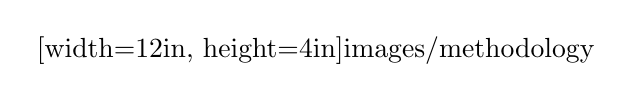
\begin{tikzpicture}[remember picture]
    \node[anchor=north west]
        at (current page.north west) {
        \includesvg[width=12in, height=4in]{images/methodology}
    };
    \end{tikzpicture}
  \end{center}
\end{wrapfigure}

\hspace{1cm}
\begin{latin}\textbf{Iterative Design:}\end{latin}
طراحی تکراری یک روش طراحی است که بر اساس یک فرآیند چرخه‌ای نمونه‌سازی، آزمایش، تجزیه و تحلیل و پالایش یک محصول یا فرآیند است. بر اساس نتایج آزمایش جدیدترین تکرار یک طرح، تغییرات و اصلاحاتی انجام می شود. این فرآیند در نهایت برای بهبود کیفیت و عملکرد یک طراحی در نظر گرفته شده است. در طراحی تکراری، تعامل با سیستم طراحی شده به عنوان شکلی از تحقیق برای اطلاع رسانی و تکامل یک پروژه استفاده می شود، زیرا نسخه های متوالی یا تکرار یک طرح اجرا می شود.
